\chapter{Arquitetura física}


\section{Uso de memória}


\section{Diagrama de objetos}

O diagrama apresentado na figura \ref{fig:objetos} representa os objetos e a comunicação entre eles no sistema.

\begin{figure}[h]
    \centering
    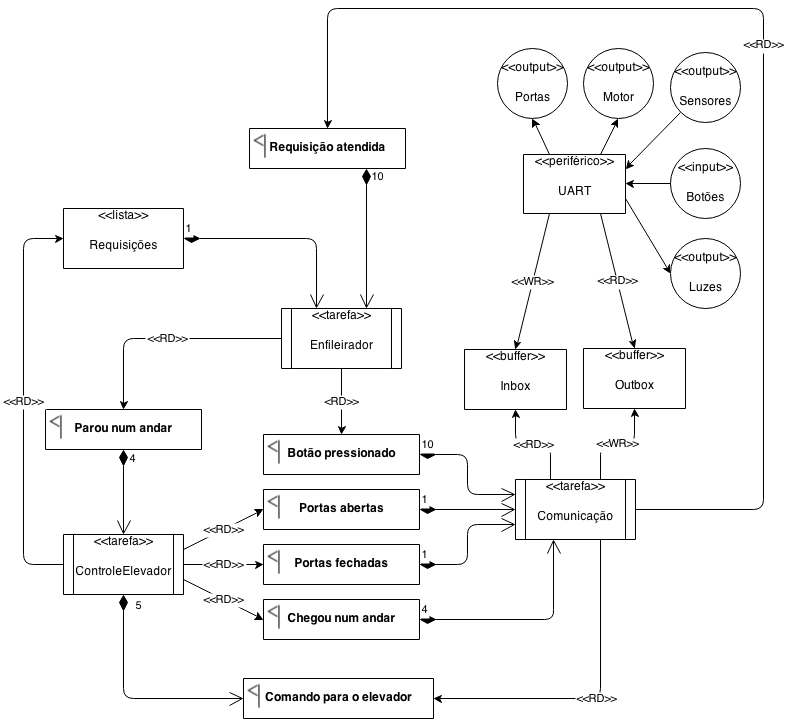
\includegraphics[width=0.8\columnwidth]{./figures/Objetos.png}
    \caption{Diagrama de objetos do sistema.}
    \label{fig:objetos}
\end{figure}

Os objetos Botões, Luzes, Portas, Sensores e Motor são objetos externos ao sistema, colocados no diagrama para indicar o interfaceamento externo do sistema.

Os sinais "Botão pressionado" indicam que o botão correspondente foi pressionado.

Os sinais "Requisição atendida" indicam que a requisição correspondente foi atendida e o sistema deve apagar a luz correspondente.

O sinal "Porta aberta" indica que as portas foram completamente abertas.

O sinal "Porta fechada" indica que as portas foram completamente fechadas.

Os sinais "Chegou num andar" indicam que o elevador chegou no andar correspondente.

Os sinais "Comando para o elevador" indicam um dos comandos possíveis para o elevador: Subir; Descer; Parar; Abrir portas; Fechar portas.

Os sinais "Parou num andar" indicam que o elevador parou no andar correspondente.

A tarefa Comunicação é responsável por fazer o interfaceamento interno ao sistema, através de um periférico de comunicação serial. Esta tarefa faz a leitura dos dados recebidos pela UART e transforma em sinais para serem usados pelas outras duas tarefas. Ela também recebe comandos para controle do elevador da tarefa ControleElevador e envia pela UART para o sistema externo.

A tarefa Enfileirador é responsável por colocar e remover as requisições em uma fila.

A tarefa ControleElevador é responsável por decidir sobre o movimento do elevador e a abertura e fechamento das portas.

% TODO: colocar figura do diagrama de estados

